%!TEX root = ../template.tex
%%%%%%%%%%%%%%%%%%%%%%%%%%%%%%%%%%%%%%%%%%%%%%%%%%%%%%%%%%%%%%%%%%%%%%
%% options.tex
%% NOVA thesis configuration file
%%
%% Processing of Class options
%%
%% Order and language for printing the abstracts depending on the language
%% These macros are just informative for now (it is hardcoded in the
%% 	novathesis.ldf file)… this must be fixed in the future!!
%%%%%%%%%%%%%%%%%%%%%%%%%%%%%%%%%%%%%%%%%%%%%%%%%%%%%%%%%%%%%%%%%%%%%%
%!TEX root = ../template.tex
%%%%%%%%%%%%%%%%%%%%%%%%%%%%%%%%%%%%%%%%%%%%%%%%%%%%%%%%%%%%%%%%%%%%%%
%% options.tex
%% NOVA thesis configuration file
%%
%% Processing of Class options
%%
%% Order and language for printing the abstracts depending on the language
%% These macros are just informative for now (it is hardcoded in the
%% 	novathesis.ldf file)… this must be fixed in the future!!
%%%%%%%%%%%%%%%%%%%%%%%%%%%%%%%%%%%%%%%%%%%%%%%%%%%%%%%%%%%%%%%%%%%%%%

\typeout{NT LOADING FILE options.tex}

%%%%%%%%%%%%%%%%%%%%%%%%%%%%%%%%%%%%%%%%%%%%%%%%%%%%%%%%%%%%%%%%%%%%%%%%
%% PROCESS KEY-VAL OPTIONS
%%%%%%%%%%%%%%%%%%%%%%%%%%%%%%%%%%%%%%%%%%%%%%%%%%%%%%%%%%%%%%%%%%%%%%%%%
\RequirePackage{options-nt}
\RequirePackage{xifthen}
\options{/@nt/.new family
  % languages
  , langsshort/.new list = {pt, en, fr, it}
  , langslong/.new list = {portuguese, english, french, italian}
  , langshorttolong/.new choice = {pt=portuguese, en=english, fr=french, 
                                   it=italian}
  , maplang/.new cmd = {%
            \options{/@nt/langshorttolong = #1}%
            \option{/@nt/langshorttolong}%
  }  
  % %novathesis@opt@biblatex
  , biblatex/.new list
  , handler/school/.new cmd = {%
            \typeout{NT HANDLER SCHOOL ROUTINE [#1]}
            \ifoptiondefined{/@nt/cover/\option{/novathesis/school}/element}%
              {}% it as a reload… do nothing
              {% Load new school definitions
                \prependtographicspath{{NOVAthesisFiles/Schools/#1/Images/}}%
                \InputIfFileExists{NOVAthesisFiles/Schools/#1/defaults.ldf}%
                  {}%
                  {\PackageWarining{novathesis}%
                                   {Missing file “defaults.ldf” for #1}}%
              }%
  }
  , handler/media/.new cmd = {%
              \setulmarginsandblock%
                {\themargin[#1,top]}%
                {\themargin[#1,bottom]}%
                {*}%
              \setlrmarginsandblock%
                {\themargin[#1,left]}%
                {\themargin[#1,right]}%
                {*}%
              \checkandfixthelayout%
              \ifthenelse{\equal{\option{/novathesis/media}}{paper}}%
                {\options{/novathesis/linkscolor=black}}
                {}
  }
  , handler/chapstyle/.new cmd = {%
    \InputIfFileExists{NOVAthesisFiles/ChapStyles/#1.ldf}{}%
      {\PackageWarining{novathesis}{Invalid Chapter Style: #1}}
  }
  , handler/fontstyle/.new cmd = {%
    \InputIfFileExists{NOVAthesisFiles/FontStyles/#1.ldf}{}%
      {\PackageWarining{novathesis}{Invalid Font Style: #1}}
  }
}

\options{/novathesis/.new family
  % %novathesis@opt@docdegree
  , docdegree/.new choice = {phd, phdprop, phdplan, msc, mscplan, bsc},
  % %novathesis@opt@school
  , school/.new choice = {{nova/fct}, {nova/fcsh}, {nova/ims}, {nova/ensp},
                          {ul/ist}, {ul/fc}, {ipl/isel}, {ips/ests}, {esep}}
  % %novathesis@opt@chapstyle
  , chapstyle/.new choice = {bianchi, bluebox, default, elegant, 
                             ell, hansen, ist, lyhne, madsen,
                            pedersen, section, southall, veelo,
                            vz34, vz43}
  , chapstyle=elegant        % set elegant as the default
  % %novathesis@opt@fontstyle
  , fontstyle/.new choice = {kpfonts, bookman, erewhon, libertine, scholax,
                             calibri, kieranhealy}
  , fontstyle=kpfonts        % set kpfonts as the default
  % HANDLER
  , lang/.new style = {/novathesis/mainlang=#1,/novathesis/copyrightlang=#1,
                       /novathesis/coverlang=#1}
  % %novathesis@opt@lang
  , mainlang/.new choice = {pt, en, fr, it}
  % %novathesis@opt@coverlang
  , coverlang/.new choice = {pt, en, fr, it}
  % %novathesis@opt@copyrightlang
  , copyrightlang/.new choice = {pt, en, fr, it}
  % %novathesis@opt@printcommittee
  , printcommittee/.new toggle = true
  % %novathesis@opt@secondcover
  , secondcover/.new toggle = false
  % %novathesis@opt@aftercover
  , aftercover/.new toggle = false
  , urlstyle/.new cmd = {%
            \edef\@nt@urlstyle{#1}\AfterPreamble{\urlstyle{\@nt@urlstyle}}%
  }
  , debugcover/.new toggle = false
  , spine/.new cmd* = {%
            \AtEndDocument{%
              \InputIfFileExists{%
                  NOVAthesisFiles/Schools/\option{/novathesis/school}/spine.tex%
              }%
                {}%
                {%%%%%%%%%%%%%%%%%%%%%%%%%%%%%%%%%%%%%%%%%%%%%%%%%%%%%%%%%%%%%%%%%%%%
%% spine.tex
%% NOVA thesis document template
%%
%% This work is licensed under the
%% The LaTeX project public license (LPPL), version 1.3c
%% To view a copy of this license, visit
%% https://www.latex-project.org/lppl/lppl-1-3c/
%%
%% Authors / Contributors:
%%      - João Lourenço <joao.lourenco@fct.unl.pt>
%%%%%%%%%%%%%%%%%%%%%%%%%%%%%%%%%%%%%%%%%%%%%%%%%%%%%%%%%%%%%%%%%%%%%

\typeout{NT FILE spine.tex}%

% Draw the book spine
% usable range: 145 to 425 pages, maximum characters for the title 140 and 22 for the author name
% usable range: 75 to 145 pages, maximum characters for the title 70 and 22 for the author name

\makeatletter

%=================================================================
% From https://tex.stackexchange.com/questions/26002/fit-text-into-given-box-by-adjusting-the-fontsize

\RequirePackage{fp}

\newcommand{\fitboxratio}[4]{%
  % #1 = ratio
  % #2 = width
  % #3 = height
  % #4 = text
  \@tempdima#3%
  \edef\@wd{\strip@pt\dimexpr#2\relax}%
  \@temptokena={\mbox{#4}}%
  \setbox0=\hbox{\the\@temptokena}%
  \@tempdimb=\dimexpr\ht0+\dp0\relax%
  \typeout{SPINE DIV1 [{\strip@pt\@tempdima}] [{\strip@pt\@tempdimb}]}%
  \FPdiv\vr@tio{\strip@pt\@tempdima}{\strip@pt\@tempdimb}%
  \@tempdimc=\dimexpr\wd0\relax%
  \FPdiv\hr@tio{\@wd}{\strip@pt\@tempdimc}%
  \typeout{SPINE DIV2 [{\@wd}] [{\strip@pt\@tempdimc}]}%
  \FPmin\r@tio{\hr@tio}{\vr@tio}%
  \def#1{\r@tio}%
  \ignorespaces%
}

\newcommand{\fitboxprint}[2]{%
  \scalebox{#1}{#2}%\ignorespaces
}

\newcommand{\fitboxmin}[2]{%
  \gdef#1{99999999}%
  \@for\@fbx:={#2}\do{%
    \FPmin#1{\@fbx}{#1}%
  }%
}

\newcommand{\fitbox}[3]{%
  % #1 = width
  % #2 = height
  % #3 = text
  \@tempdima#2%
  \edef\@wd{\strip@pt\dimexpr#1\relax}%
  \@temptokena={\mbox{#3}}%
  \setbox0=\hbox{\the\@temptokena}%
  \@tempdimb=\dimexpr\ht0+\dp0\relax%
  \FPdiv\vr@tio{\strip@pt\@tempdima}{\strip@pt\@tempdimb}%
  \@tempdimc=\dimexpr\wd0\relax%
  \FPdiv\hr@tio{\@wd}{\strip@pt\@tempdimc}%
  \FPmin\r@tio{\hr@tio}{\vr@tio}%
  \setbox0=\hbox{\scalebox{\r@tio}{#3}}%
  \box0%
}


\def\def@ult#1(#2)=#3{\ifdatadefined{#1}(#2){}{\csname#1\endcsname(#2)={#3}}}

\def@ult{spine}(author)={\thedocauthor(name,short)}
\ifdatadefined{doctitle}(\option{/novathesis/lang/cover},sub){%
  \def@ult{spine}(title)={\thedoctitle(\option{/novathesis/lang/cover},spine): \thedoctitle(\option{/novathesis/lang/cover},sub)}
}{%
  \def@ult{spine}(title)={\thedoctitle(\option{/novathesis/lang/cover},spine)}
}
% \typeout{SPINE=[\option{/novathesis/lang/cover}][\thespine(title)]}
\def@ult{spine}(date)={\thentdocdate(year)}

\def@ult{spine}(text,angle)={90}
% \def@ult{spine}(text,color)={white}
% \def@ult{spine}(box,color)={blue}
\def@ult{spine}(box,spacing)={0.5cm}
\def@ult{spine}(box,margin)={0.0cm}

\def@ult{spine}(box,logo,top)={0.0cm}
\def@ult{spine}(box,logo,len)={4.1cm}
\def@ult{spine}(box,logo,align)={c}

\def@ult{spine}(box,author,top)={\dimexpr\thespine(box,logo,top)+\thespine(box,logo,len)+\thespine(box,spacing)}
\def@ult{spine}(box,author,len)={4.0cm}

\def@ult{spine}(box,title,top)={\dimexpr\thespine(box,author,top)+\thespine(box,author,len)+\thespine(box,spacing)}
\def@ult{spine}(box,title,len)={16.7cm}
% \spine(box,title,align)={l}
% \spine(box,author,align)={l}

\def@ult{spine}(box,date,top)={\dimexpr\thespine(box,title,top)+\thespine(box,title,len)+\thespine(box,spacing)}
\def@ult{spine}(box,date,len)={2.0cm}
% \spine(box,lodatego,align)={l}

\def@ult{spine}(logo,\option{/novathesis/doctype},angle)={0}
\def@ult{spine}(logo,\option{/novathesis/doctype},raise)={0pt}
\def@ult{spine}(logo,\option{/novathesis/doctype},scale)={1}

\def@ult{spine}(logo,angle)={0}
\def@ult{spine}(logo,raise)={0pt}
\def@ult{spine}(logo,scale)={1}

\datamatchtf{\match}{thesiscover}({\option{/novathesis/doctype},spine,bgcolor},{spine,bgcolor})%
                {}%
                {\def@ult{thesiscover}(spine,framecolor)={black!20}}

\ifdatadefined{spine}(author){%
  \spine(text,author,len)={\dimexpr\thespine(box,author,len)-\thespine(box,margin)-\thespine(box,margin)}
}{}
\ifdatadefined{spine}(title){%
  \spine(text,title,len)={\dimexpr\thespine(box,title,len)-\thespine(box,margin)-\thespine(box,margin)}
}{}
\ifoptionvoid{/novathesis/degreeacr}{}{%
  \ifdatadefined{spine}(box,degreeacr,len){%
    \spine(text,degreeacr,len)=%
      {\dimexpr\thespine(box,degreeacr,len)-\thespine(box,margin)-\thespine(box,margin)}
  }{}%
}
\ifdatadefined{spine}(date){%
  \spine(text,date,len)={\dimexpr\thespine(box,date,len)-\thespine(box,margin)-\thespine(box,margin)}
}{}


\newcommand{\@spinetextalin}[1]{%
  \raggedright%
  \IfStrEqCase{\thespine(box,#1,align)}{%
    {l}{\raggedright}%
    {c}{\centering}%
    {r}{\raggedleft}%
  }%
}

\newcommand{\@spinetextcolor}[1]{%\option{/novathesis/doctype},
  \datamatchtf{\arg}{spine}({box,#1,textcolor},{box,textcolor}){\color{\arg}}{}%
}

\newcommand{\@ntprintspine}{%
  \sffamily%
  \normalsize%
  \newlength{\novathesis@spinewidth}%
  \setlength{\novathesis@spinewidth}{\dimexpr1mm * (\thelastsheet+ 19) / 20}%
  \ifdim\novathesis@spinewidth < 6mm\relax% Force book spine to be at least 6mm
    \setlength{\novathesis@spinewidth}{6mm}%
  \fi%
  \newlength{\novathesis@boxwidth}%
  \setlength{\novathesis@boxwidth}{\dimexpr\novathesis@spinewidth-1mm}%
  \newlength{\novathesis@spinetextwidth}%
  \setlength{\novathesis@spinetextwidth}%
            {\dimexpr\novathesis@boxwidth-\thespine(box,margin)-\thespine(box,margin)}%

  \ifdatadefined{spine}(title){%
    \fitboxratio{\@titleRT}{\thespine(text,title,len)}{\novathesis@spinetextwidth}
                {\thespine(title)}
  }{\def\@titleRT{99999}}%
  \ifdatadefined{spine}(author){%
    \fitboxratio{\@authorRT}{\thespine(text,author,len)}{\novathesis@spinetextwidth}
                {\thespine(author)}
  }{\def\@authorRT{99999}}%
  \ifdatadefined{spine}(date){%
    \fitboxratio{\@dateRT}{\thespine(text,date,len)}{\novathesis@spinetextwidth}
                {\thespine(date)}
  }{\def\@titleRT{99999}}%

  \fitboxmin{\@fbratio}{\@authorRT,\@titleRT,\@dateRT}%
  % \show\@authorRT
  % \show\@titleRT
  % \show\@dateRT
  % \show\@fbratio

  \defifundef{\myauthorbox}{\newsavebox}%
  \ifdatadefined{spine}(author){%
    \begin{lrbox}{\myauthorbox}%
      \begin{minipage}[c][\novathesis@spinetextwidth][c]{\thespine(text,author,len)}%
          \@spinetextalin{author}%
          \@spinetextcolor{author}%
          \fitboxprint{\@fbratio}{\thespine(author)}%
      \end{minipage}%
    \end{lrbox}%
  }{}%
  \defifundef{\mytitlebox}{\newsavebox}%%
  \ifdatadefined{spine}(title){%
    \begin{lrbox}{\mytitlebox}%
      \begin{minipage}[c][\novathesis@spinetextwidth][c]{\thespine(text,title,len)}%
          \@spinetextalin{title}%
          \@spinetextcolor{title}%
          \fitboxprint{\@fbratio}{\thespine(title)}%
      \end{minipage}%
    \end{lrbox}%
  }{}%
  \defifundef{\mydatebox}{\newsavebox}%%
  \ifdatadefined{spine}(date){%
    \begin{lrbox}{\mydatebox}%
      \begin{minipage}[c][\novathesis@spinetextwidth][c]{\thespine(text,date,len)}%
          \@spinetextalin{date}%
          \@spinetextcolor{date}%
          \fitboxprint{\@fbratio}{\thespine(date)}%
      \end{minipage}%
    \end{lrbox}%
  }{}%
  \ifoptionvoid{/novathesis/degreeacr}{}{%
    \defifundef{\mydegreeacrbox}{\newsavebox}%%
    \begin{lrbox}{\mydegreeacrbox}%
      \ifdatadefined{spine}(box,degreeacr,len){%
          \@spinetextalin{degreeacr}%
          \@spinetextcolor{degreeacr}%
          \ifdatadefined{degreeacr}(\option{/novathesis/degreeacr}){%
            \fitboxprint{\@fbratio}{\MakeTextUppercase{\thedegreeacr(\option{/novathesis/degreeacr})}}%
          }{%
            \fitboxprint{\@fbratio}{\MakeTextUppercase{\option{/novathesis/degreeacr}}}%
          }
      }{}%
    \end{lrbox}%
  }%

  % \options{/@ntcoveropts/bookmark=spine}%
  \currentpdfbookmark{sipne}{\@LANG@COVER}%
  \ifoptionequal{/novathesis/spine}{trim}{%
    \setstocksize{\paperheight}{\novathesis@spinewidth}
    \settrimmedsize{\stockheight}{\stockwidth}{*}%
    \setlrmarginsandblock{0pt}{0pt}{*}%
    \setulmarginsandblock{0pt}{*}{1}%
    \setheadfoot{0pt}{0pt}%
    \setheaderspaces{0pt}{*}{*}%
    \checkandfixthelayout[fixed]%
    \ifluatex
        \pagewidth=\novathesis@spinewidth% \pageheight=3in
    \else
        \pdfpagewidth=\novathesis@spinewidth% \pdfpageheight=3in
    \fi
  }{}%
  \thispagestyle{empty}%
  \NTRunHook{spine/pre}%
  \begin{tikzpicture}[remember picture, overlay]
  % draw image
    % print bg color IF DEFINED
    \datamatchtf{\arg}{thesiscover}(%
                      {\option{/novathesis/doctype},spine,bgcolor},%
                      {\option{/@nt/document/docclass},spine,bgcolor},%
                      {spine,bgcolor},%
                      {bgcolor}%
    ){%
      \node[inner sep=0, anchor=center,
            rectangle, minimum width=\novathesis@spinewidth, minimum height=\paperheight,
            fill=\arg]
           at (current page.center)
              {};
    }{}%
    % print frame IF DEFINED
    \datamatchtf{\arg}{thesiscover}(%
                      {\option{/novathesis/doctype},spine,framecolor},%
                      {\option{/@nt/document/docclass},spine,framecolor},%
                      {spine,framecolor},%
                      {framecolor}%
    ){%
      \node[inner sep=0, anchor=center,
            rectangle, minimum width=\novathesis@spinewidth, minimum height=\paperheight,
            draw=\arg,fill=none]
           at (current page.center)
              {};
    }{}%
    % print bg image IF DEFINED
    \datamatchtf{\arg}{thesiscover}(%
                      {\option{/novathesis/doctype},spine,image},%
                      {\option{/@nt/document/docclass},spine,image},%
                      {spine,image},%
                      {image}%
    ){%
      \node[inner sep=0] at (current page.center)
              {\includegraphics[width=\novathesis@spinewidth,height=\paperheight]{\arg}};
    }{}%
    % print logo IF DEFINED
    \datamatchtf{\arg}{spine}(%
                      {logo,\option{/novathesis/doctype}},%
                      {logo,\option{/@nt/document/docclass}},%
                      {logo}%
    ){%
      \datamatchtf{\@angle}{spine}(%
                        {logo,\option{/novathesis/doctype},angle},%
                        {logo,\option{/@nt/document/docclass},angle},%
                        {logo,angle}%
      ){}{\def\@angle{0}}%
      \datamatchtf{\@scale}{spine}(%
                        {logo,\option{/novathesis/doctype},scale},%
                        {logo,\option{/@nt/document/docclass},scale},%
                        {logo,scale}%
      ){}{\def\@scale{1}}%
      \datamatchtf{\@raise}{spine}(%
                        {logo,\option{/novathesis/doctype},raise},%
                        {logo,\option{/@nt/document/docclass},raise},%
                        {logo,raise}%
      ){}{\def\@raise{0pt}}%
      \node[inner sep=0, anchor=center,
            yshift=-\dimexpr\expanded{\thespine(box,logo,top)+(\thespine(box,logo,len)/2)},
            xshift=-\novathesis@boxwidth*\@raise,
           ]
           at (current page.north)
              {\defifundef{\logobox}{\newsavebox}%
               \defifundef{\logoboxht}{\newlength}%
               \IfStrEq{\@angle}{0}{%
                 \savebox{\logobox}{\includegraphics[width=\novathesis@boxwidth,
                                                     angle=\@angle,
                                                     scale=\@scale]{\arg}}%
                 \settoheight{\logoboxht}{\usebox{\logobox}}%
                 \ifdim\logoboxht>\thespine(box,logo,len)\relax
                   \savebox{\logobox}{\includegraphics[height={\thespine(box,logo,len)},
                                                     angle=\@angle,
                                                     scale=\@scale]{\arg}}%
                 \fi
               }{%
                 \savebox{\logobox}{\includegraphics[height=\novathesis@boxwidth,
                                                     angle=\@angle,
                                                     scale=\@scale]{\arg}}%
                 \settoheight{\logoboxht}{\usebox{\logobox}}%
                 \ifdim\logoboxht>\thespine(box,logo,len)\relax
                   \savebox{\logobox}{\includegraphics[width={\thespine(box,logo,len)},
                                                     angle=\@angle,
                                                     scale=\@scale]{\arg}}%
                 \fi
               }%
               {\usebox{\logobox}}%
               % \includegraphics[angle=\@angle, scale=\@scale, align=c]{\arg}%
              };
    }{}%
    % print author
    \ifdatadefined{spine}(author){%
      \datamatchtf{\@fcolor}{spine}({box,author,color},{box,color}){}{\gdef\@fcolor{none}}%
      \node[inner sep=0, anchor=north, yshift=-(\dimexpr\expanded{\thespine(box,author,top)})
            , rectangle, minimum width=\novathesis@boxwidth, minimum height=\expanded{\thespine(box,author,len)}
            , fill=\@fcolor]
           at (current page.north)
              {\rotatebox{\thespine(text,angle)}{\hspace*{\thespine(box,margin)}\usebox{\myauthorbox}}};
    }{}
    % print title
    \ifdatadefined{spine}(title){%
      \datamatchtf{\@fcolor}{spine}({box,title,color},{box,color}){}{\gdef\@fcolor{none}}%
      \node[inner sep=0, anchor=north, yshift=-(\dimexpr\expanded{\thespine(box,title,top)})
            , rectangle, minimum width=\novathesis@boxwidth, minimum height=\expanded{\thespine(box,title,len)}
            , fill=\@fcolor]
           at (current page.north)
              {\rotatebox{\thespine(text,angle)}{\hspace*{\thespine(box,margin)}\usebox{\mytitlebox}}};
    }{}
    % print degree IF DEFINED
    \ifoptionvoid{/novathesis/degreeacr}{}{%
      \ifdatadefined{spine}(box,degreeacr,len){%
        \datamatchtf{\@fcolor}%
                    {spine}({box,degreeacr,color},{box,color}){}{\gdef\@fcolor{none}}%
        \node[inner sep=0,anchor=north, yshift=-\dimexpr\expanded{\thespine(box,degreeacr,top)}
              , rectangle,minimum width=\novathesis@boxwidth, minimum height=\expanded{\thespine(box,degreeacr,len)}
              , fill=\@fcolor]
             at (current page.north)
                {\rotatebox{\thespine(text,angle)}{\usebox{\mydegreeacrbox}}};
      }{}%
    }
    % print date
    \ifdatadefined{spine}(date){%
      \datamatchtf{\@fcolor}{spine}({box,date,color},{box,color}){}{\gdef\@fcolor{none}}%
      \node[inner sep=0,anchor=north, yshift=-(\dimexpr\expanded{\thespine(box,date,top)})
            , rectangle,minimum width=\novathesis@boxwidth, minimum height=\expanded{\thespine(box,date,len)}
            , fill=\@fcolor]
           at (current page.north)
              {\rotatebox{\thespine(text,angle)}{\usebox{\mydatebox}}};
    }{}
  \end{tikzpicture}
  \ifoptioncontains{/novathesis/debug}{cover}{\debuggrid}{}%
  \NTRunHook{spine/post}%
}
}%
              \ntprintspine%
            }%
  }
  % %novathesis@opt@cdcover
  , cdcover/.new cmd* = {%
            \AtEndDocument{%
            \InputIfFileExists{%
                NOVAthesisFiles/Schools/\option{/novathesis/school}/cdcover.tex%
            }%
              {}%
              {%!TEX root = ../template.tex
%%%%%%%%%%%%%%%%%%%%%%%%%%%%%%%%%%%%%%%%%%%%%%%%%%%%%%%%%%%%%%%%%%%%
%% cdcover.tex
%% NOVA thesis document template
%%
%% This work is licensed under the
%% The LaTeX project public license (LPPL), version 1.3c
%% To view a copy of this license, visit
%% https://www.latex-project.org/lppl/lppl-1-3c/
%%
%% Authors / Contributors:
%%      - João Lourenço <joao.lourenco@fct.unl.pt>
%%      - Tomás Monteiro <monteiro.tomas@gmail.com>
%%
%% This CD cover is a refactoring of the pull request by Tomás Monteiro
%% to reuse the information already provided in the file “template.tex”
%%%%%%%%%%%%%%%%%%%%%%%%%%%%%%%%%%%%%%%%%%%%%%%%%%%%%%%%%%%%%%%%%%%%%

\typeout{NT LOADING FILE cdcover.tex}


% Draw the cdcover


%% Cover: 12.0cm x 12.0cm
%% Inlay: 15.0cm x 11.8cm
%% Inlay fold: 0,635cm + 13,73cm + 0,635cm

\typeout{NT LOADING FILE cdcolver.ldf}

\makeatletter

\prependtographicspath{{NOVAthesisFiles/Images/}}

\newsavebox{\cdcover@savebox}

\newcommand{\ntprintcdcover}{%
	\clearpage

	\thispagestyle{empty}
	\pagestyle{empty}
	
	\setstocksize{12cm}{12cm}
	\settrimmedsize{\stockheight}{\stockwidth}{*}
	\settrims{0pt}{0pt}
	\setlrmarginsandblock{*}{-5mm}{*}
	\setulmarginsandblock{0mm}{*}{*}
	% \setlength{\parskip}{0pt}
	\setheadfoot{0mm}{0mm}
	\setheaderspaces{*}{0mm}{*}
	\setmarginnotes{0mm}{0mm}{0mm}
	\checkandfixthelayout[fixed]

  \AddToShipoutPictureBG*{
\includegraphics[width=120mm]{cd-cover-std}}

	\savebox{\cdcover@savebox}{%
	\begin{minipage}[t][7.0cm]{9cm}
		
		% Author name
		% \raggedright
		% \raggedleft
		\centering
		\fontsize{12}{12}\selectfont
		\textbf{\theauthorname}
		\medskip

		% Academic qualifications
		\fontsize{9}{9}\selectfont
		\theauthordegree
		\vfill

		% Title of Dissertation
		\fontsize{12}{12}\selectfont
		\textbf{\thetitle}
		\vfill

		% Degree
		\fontsize{9}{9}\selectfont
		\thepresentationtext
		\vfill

		% Date
		\fontsize{9}{9}\selectfont
		\textbf{\thentdatemonth, \thentdateyear}	
		
		
	\end{minipage}
	}

	~\\[1.75cm]~\hspace*{1.7cm}
	\usebox{\cdcover@savebox}

}

\newcommand{\ntprintcdinlay}{%
	\clearpage

	\thispagestyle{empty}
	\pagestyle{empty}
	
	\setstocksize{11.8cm}{15cm}
	\settrimmedsize{\stockheight}{\stockwidth}{*}
	\settrims{0pt}{0pt}
	\setlrmarginsandblock{*}{0mm}{*}
	\setulmarginsandblock{0mm}{*}{*}
	% \setlength{\parskip}{0pt}
	\setheadfoot{0mm}{0mm}
	\setheaderspaces{*}{0mm}{*}
	\setmarginnotes{0mm}{0mm}{0mm}
	\checkandfixthelayout[fixed]

  \AddToShipoutPictureBG*{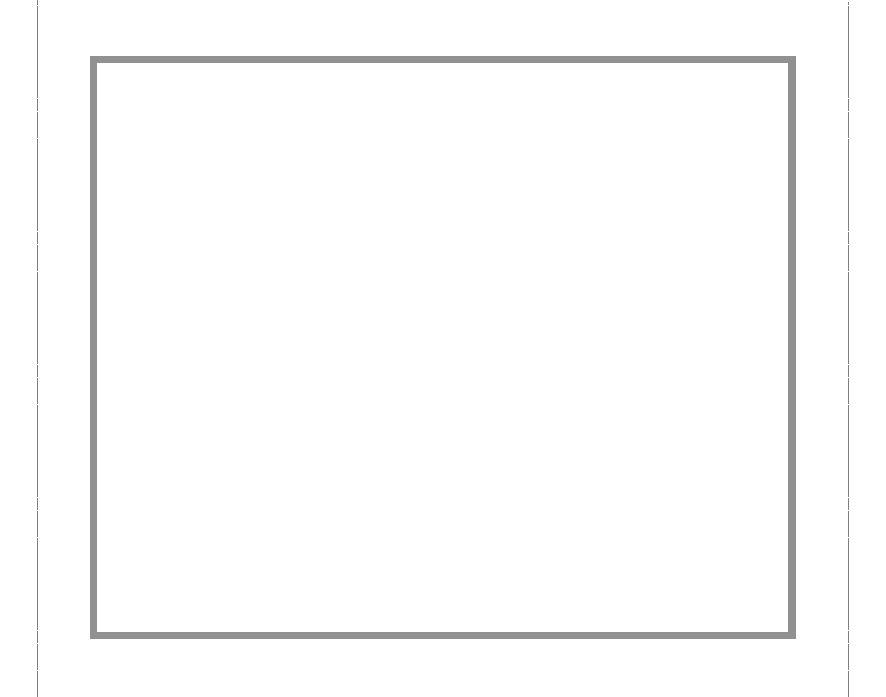
\includegraphics[width=150mm]{cd-inlay-std}}

	\savebox{\cdcover@savebox}{%
	\begin{minipage}[t][8cm]{11cm}
		
		% Author name
		% \raggedright
		% \raggedleft
		{
		\centering
		\vfill
		\fontsize{12}{12}\selectfont
		\textbf{\theauthorname}
		\medskip

		% Academic qualifications
		\fontsize{9}{9}\selectfont
		\theauthordegree
		\vfill

		% Title of Dissertation
		\fontsize{12}{12}\selectfont
		\textbf{\thetitle}
		\vfill

		% Degree
		\fontsize{9}{9}\selectfont
		\thepresentationtext
		\vfill

		% Date
		\fontsize{9}{9}\selectfont
		\textbf{\thentdatemonth, \thentdateyear}	
		\vfill

		}
		\fontsize{5}{7}\selectfont
		\thecopyrightstr
		
	\end{minipage}
	}
	
	\par

	\setlength{\fboxsep}{0pt}
	% ~\hspace*{1.8cm}
	~\\[0.75cm]~\hspace*{1.8cm}
	\usebox{\cdcover@savebox}
}

\makeatother
}%
            \ntprintcdcover%  
            \ntprintcdinlay%
            }%
  }
  % %novathesis@opt@media
  , media/.new choice = {screen, paper}
  %novathesis@opt@linkscolor
  , linkscolor/.new cmd = {%
            \@ifpackageloaded{hyperref}%
              {\hypersetup{allcolors=#1}}%
              {\PassOptionsToPackage{allcolors=#1}{hyperref}}%
  }
}

\newcommand*{\ntsetup}[1]{%
  \ntgetkeyval{#1}\@nt@opt\@nt@value
  % \typeout{'NT SETUP = '[#1]~/~[\@nt@opt]~/~[\@nt@value]}
  \csuse{@nt@opt\@nt@opt @prehook}
  \options{/novathesis/\@nt@opt = {\@nt@value}}%
  % \typeout{'NT HANDLER = '/novathesis/handler/\@nt@opt}%
  \option{/@nt/handler/\@nt@opt}
  % \typeout{NT ->@nt@opt#1hook}
}

\newcommand*{\@nt@optschool@prehook}{%
}


\newcommand*{\ntbibsetup}[1]{\options{/@nt/biblatex/.push={#1}}}


% --------------------------------------------------------
% PROCESSING CLASS OPTIONS
\options@ProcessOptions{/novathesis}%


% --------------------------------------------------------
% FORCE SOME OPTIONS
\@AtEndClass{\options{/novathesis/printcommittee = false}}


% --------------------------------------------------------
% BABEL STUFF
\options@ProcessOptions{/novathesis}
\newcommand{\maplang}[1]{%
  \options{/@nt/maplang=#1}%
}

%
% % BABEL
\edef\nt@alllangs{}
\optionlistdo{/@nt/langsshort}{%
  \options{/@nt/langshorttolong=#1}%
  \ifoptionequal{/novathesis/mainlang}{#1}%
    {\edef\nt@alllangs{\nt@alllangs,main=\option{/@nt/langshorttolong}}}%
    {\edef\nt@alllangs{\nt@alllangs,\option{/@nt/langshorttolong}}}%
}
% \typeout{'NT PASSING TO BABEL = '\nt@alllangs}
\PassOptionsToPackage{\nt@alllangs}{babel}%

% --------------------------------------------------------
% Define DEFAULT VALUES for COVER and COPYRIGHT languages
\options{%
  /novathesis/coverlang = \option{/novathesis/mainlang}
  , /novathesis/copyrightlang = \option{/novathesis/mainlang}
  , /novathesis/linkscolor = RoyalBlue
}



% --------------------------------------------------------
% Pass the remaining options to memoir
\letoptionlist{/options/remaining}\nt@remaining
% \typeout{'NT PASSING TO MEMOIR='\nt@remaining}
\PassOptionsToClass{\nt@remaining}{memoir}
